\chapter{Evaluation}
In questa sezione vengono presentati i risultati delle simulazioni effettuate e i loro valori.
Ogni simulazione presenta la propria immagine che ne dimostra i risultati nella sezione \textit{Risultati delle simulazioni}\space\cref{risultati}.
\section{Simulazione 1}\label{sim1}
I valori di questa simulazione\space \cref{fig:sim1} sono i seguenti:
\begin{table}[ht]
    \centering
    \caption{Valori dei parametri}
    \begin{tabular}{ll}
        \toprule
        Parametro                   & Valore \\
        \midrule
        Numero di nodi              & 500    \\
        \texttt{sniffThreshold}     & 1.5    \\
        \texttt{wiggleBias}         & 0      \\
        \texttt{evaporation}        & 0.6    \\
        \texttt{diffusion}          & 0.5    \\
        \texttt{deposit}            & 1      \\
        \texttt{startX}             & -15    \\
        \texttt{startY}             & -15    \\
        \texttt{width}              & 30     \\
        \texttt{height}             & 30     \\
        \texttt{step}               & 0.5    \\
        \texttt{customDiffusionTreshold} & 5 \\
        \bottomrule
    \end{tabular}\label{tab:parametri1}
\end{table}\newline
Dalle dimensioni dell'ambiente si può osservare che il numero di \textit{patch} è pari a 3721, quindi 3721 punti che 
immagazzineranno la quantità di feromone depositata dai nodi. Ci si aspetta che l'aggregazione avvenga abbastanza rapidamente e in
zone definite data l'alta densità di punti di raccolta del feromone e, in generale, dell'ambiente. Con 500 nodi 
ci si aspetta che appena dei nodi sono vicini rimangano ``intrappolati'' nelle loro posizioni, depositando il feromone e 
generando un piccolo ``nucleo'' di aggregazione. Una volta formato, tutti i nodi che si trovano nelle vicinanze saranno attratti
e contriburanno a rafforzare l'aggregazione.


\section{Simulazione 2}\label{sim2}
I valori di questa simulazione\space \cref{fig:sim2} sono i seguenti:
\begin{table}[ht]
    \centering
    \caption{Valori dei parametri}
    \begin{tabular}{ll}
        \hline
        Parametro                   & Valore \\
        \hline
        Numero di nodi              & 500    \\
        \texttt{sniffThreshold}     & 4      \\
        \texttt{wiggleBias}         & 0      \\
        \texttt{evaporation}        & 0.6    \\
        \texttt{diffusion}          & $\frac{1}{18}$ \\
        \texttt{deposit}            & 1      \\
        \texttt{startX}             & -15    \\
        \texttt{startY}             & -15    \\
        \texttt{width}              & 30     \\
        \texttt{height}             & 30     \\
        \texttt{step}               & 0.5    \\
        \texttt{customDiffusionTreshold} & 1 \\
        \hline
    \end{tabular}\label{tab:parametr2}
\end{table}\newline
Questa simulazione presenta gli stessi valori della precedente, ma con un valore di \texttt{sniffThreshold} più alto e un valore di \texttt{diffusion} più basso.
Ci si aspetta che l'aggregazione avvenga più lentamente, i nodi si muovano per più tempo nello spazio prima di aggregarsi o di trovare un 
agglomerato già presente e che, generamlente, ci saranno meno zone di aggregazione: quindi quelle che ci saranno 
conterranno un grande numero di nodi. Il motivo di queste deduzioni è principalmente legato al fatto che il valore di \texttt{diffusion} è più basso rispetto alla simulazione
precedente\space\cref{sim1} e il valore di \texttt{sniffThreshold} è più alto. Sarà necessario che un maggior numero di nodi 
si incontri in un punto per formare un cluster. 

\section{Simulazione 3}\label{sim3}
I valori di questa simulazione\space \cref{fig:sim3} sono i seguenti:
\begin{table}[ht]
    \centering
    \caption{Valori dei parametri}
    \begin{tabular}{ll}
        \toprule
        Parametro                   & Valore \\
        \midrule
        Numero di nodi              & 100    \\
        \texttt{sniffThreshold}     & 1.5    \\
        \texttt{wiggleBias}         & 0      \\
        \texttt{evaporation}        & 0.6    \\
        \texttt{diffusion}          & 0.5    \\
        \texttt{deposit}            & 1      \\
        \texttt{startX}             & -15    \\
        \texttt{startY}             & -15    \\
        \texttt{width}              & 30     \\
        \texttt{height}             & 30     \\
        \texttt{step}               & 0.5    \\
        \texttt{customDiffusionTreshold} & 5 \\
        \bottomrule
    \end{tabular}\label{tab:parametri3}
\end{table}\newline
Questa simulazione dimostra che, pur con un numero di nodi estremamente inferiore rispetto alle precedenti,
l'aggregazione avviene comunque. I valori sono gli stessi della prima simulazione\space\cref{sim1}, ma con un numero di nodi pari a 100.
Si osserva che dopo 100 secondi si inizia a sviluppare un'aggregazione lieve, in pochissimi punti dello spazio.
Dopo 300 secondi si può notare che l'aggregazione si è rafforzata in quei punti, ma sono presenti ancora diversi nodi vaganti.


\section{Simulazione 4}\label{sim4}
\begin{table}[ht]
    \centering
    \caption{Valori dei parametri}
    \begin{tabular}{ll}
        \hline
        Parametro                   & Valore \\
        \hline
        Numero di nodi              & 100    \\
        \texttt{sniffThreshold}     & 4      \\
        \texttt{wiggleBias}         & 0      \\
        \texttt{evaporation}        & 0.6    \\
        \texttt{diffusion}          & $\frac{1}{18}$ \\
        \texttt{deposit}            & 1      \\
        \texttt{startX}             & -15    \\
        \texttt{startY}             & -15    \\
        \texttt{width}              & 30     \\
        \texttt{height}             & 30     \\
        \texttt{step}               & 0.5    \\
        \texttt{customDiffusionTreshold} & 1 \\
        \hline
    \end{tabular}\label{tab:parametri4}
\end{table}

Questa simulazione presenta gli stessi valori della seconda simulazione\space\cref{sim2}, ma con un numero di nodi pari a 100.
Lo scopo di questa simulazione è quello di confrontare i risultati con la terza simulazione\space\cref{sim3}, che presenta gli stessi valori della prima simulazione\space\cref{sim1},
ma con differenze nel \texttt{sniffThreshold} e \texttt{diffusion}. In questo caso non avviene alcuna aggregazione e 
il motivo principale è legato alle differenze di valori di \texttt{sniffThreshold} e \texttt{diffusion}.

I valori di questa simulazione\space \cref{fig:sim4} sono i seguenti:


\section{Simulazione 5}\label{sim5}
I valori di questa simulazione\space \cref{fig:sim5} sono i seguenti:
\begin{table}[ht]
    \centering
    \caption{Valori dei parametri}
    \begin{tabular}{ll}
        \hline
        Parametro                   & Valore \\
        \hline
        Numero di nodi              & 500    \\
        \texttt{sniffThreshold}     & 4      \\
        \texttt{wiggleBias}         & 0      \\
        \texttt{evaporation}        & 0.5    \\
        \texttt{diffusion}          & 1 \\
        \texttt{deposit}            & 2      \\
        \texttt{startX}             & -10    \\
        \texttt{startY}             & -10    \\
        \texttt{width}              & 20     \\
        \texttt{height}             & 20     \\
        \texttt{step}               & 0.5    \\
        \texttt{customDiffusionTreshold} & 10 \\
        \hline
    \end{tabular}\label{tab:parametri5}
\end{table}\newline
Quest'ultima simulazione presenta valori diversi da quelle precedenti. Si è voluto indagare il caso
in cui si avesse un ambiente più piccolo e dei valori di \texttt{evaporation}, \texttt{diffusion} e \texttt{deposit} 
più alti. Con questa configurazione si osserva una quasi immediata aggregazione dei nodi in tanti punti: questo comportamento
era atteso dati i valori di partenza.


\section{Risultati delle simulazioni}\label{risultati}
\begin{figure}[ht]
    \centering
    \subfigure[]{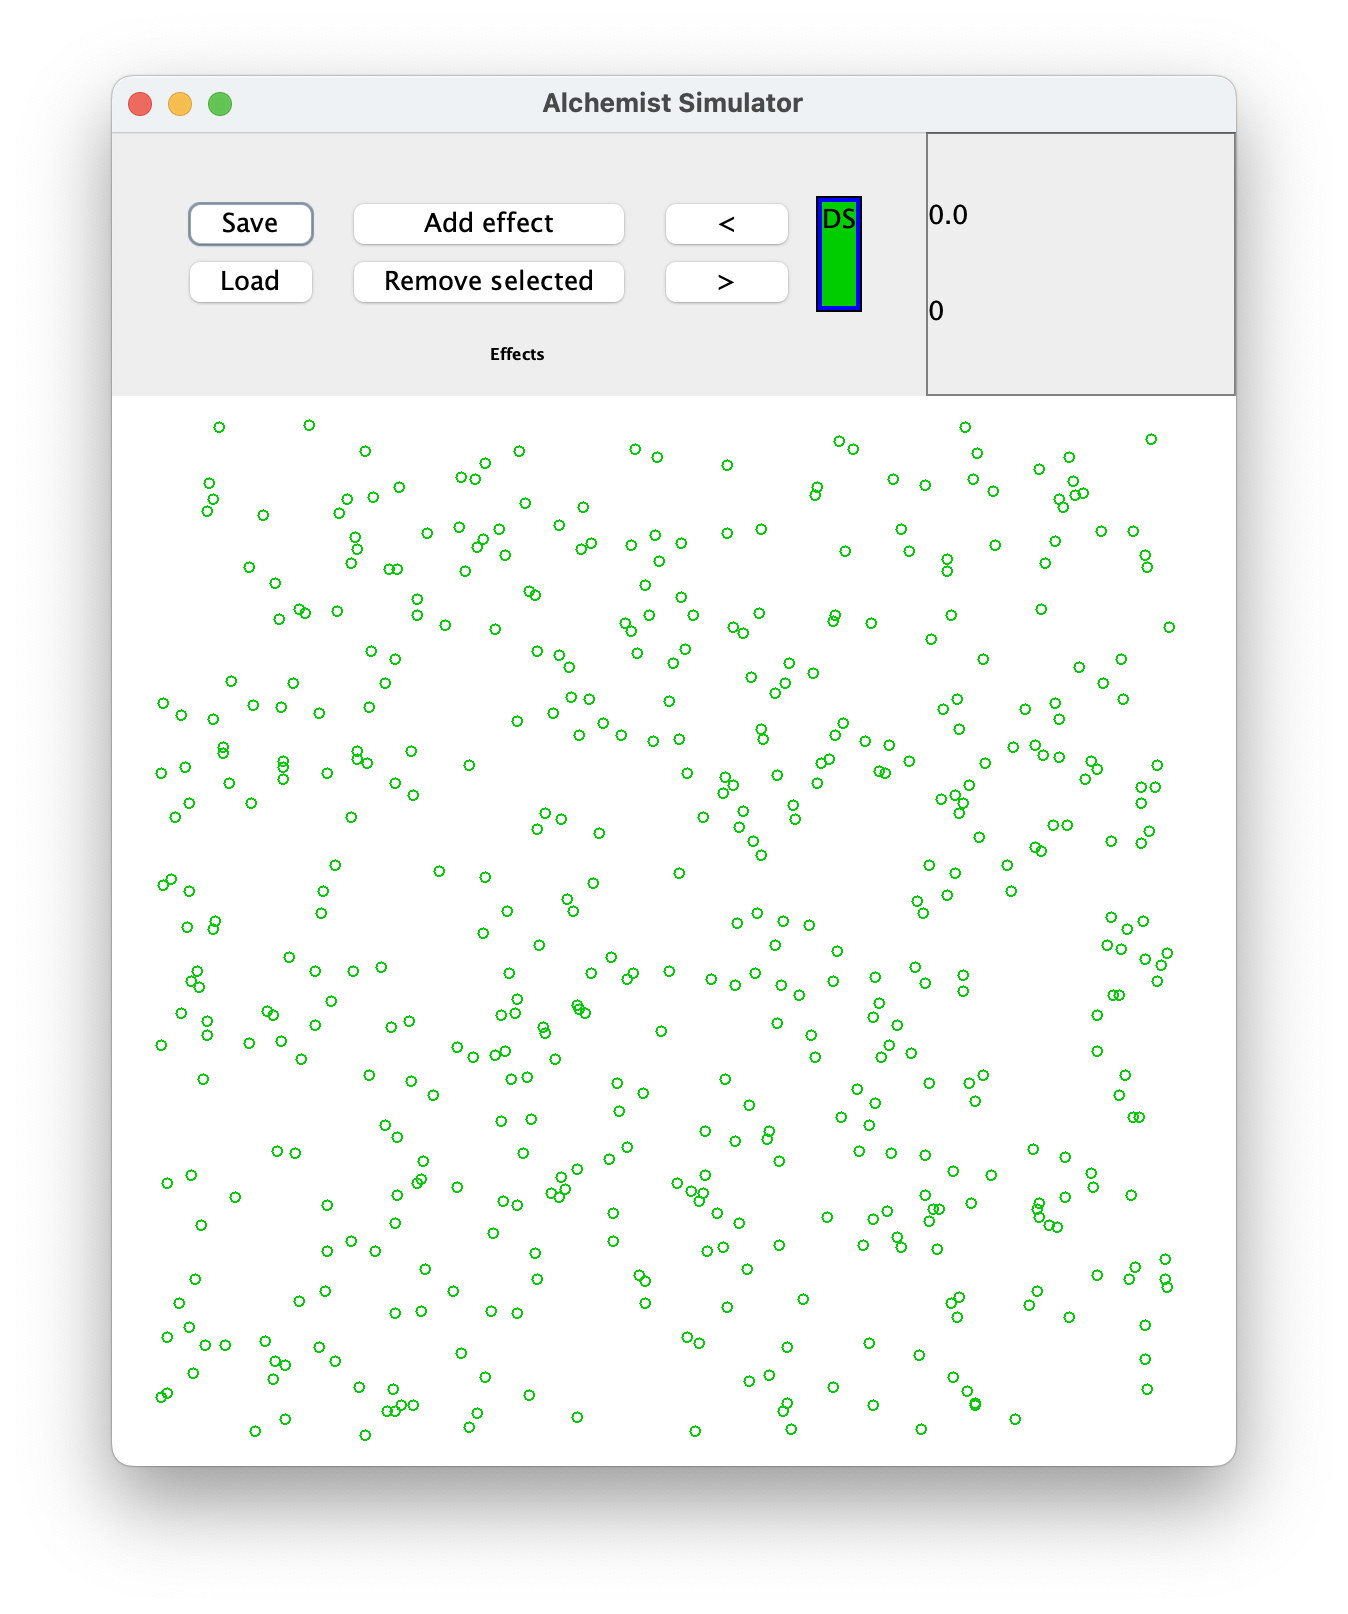
\includegraphics[width=0.32\textwidth]{figures/rect0.png}} 
    \subfigure[]{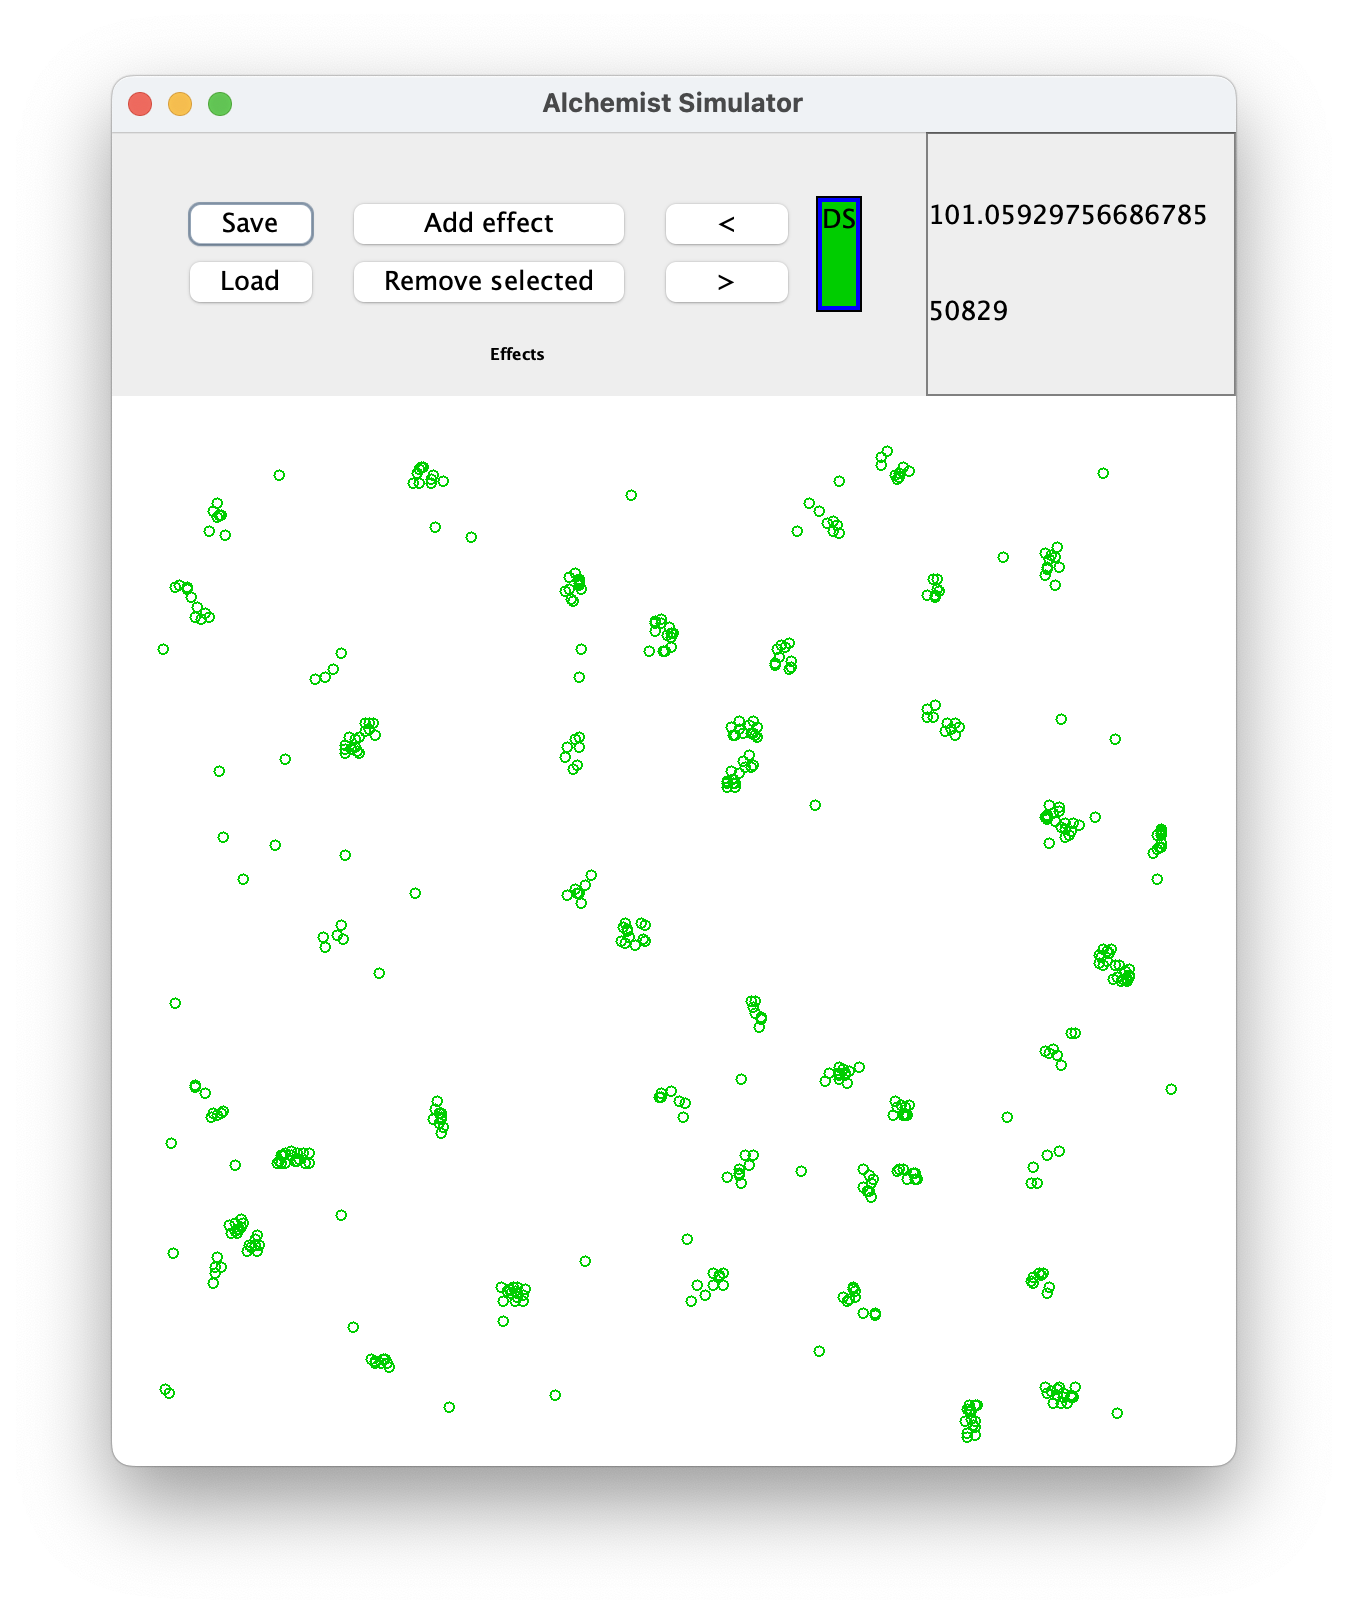
\includegraphics[width=0.32\textwidth]{figures/rect100.png}} 
    \subfigure[]{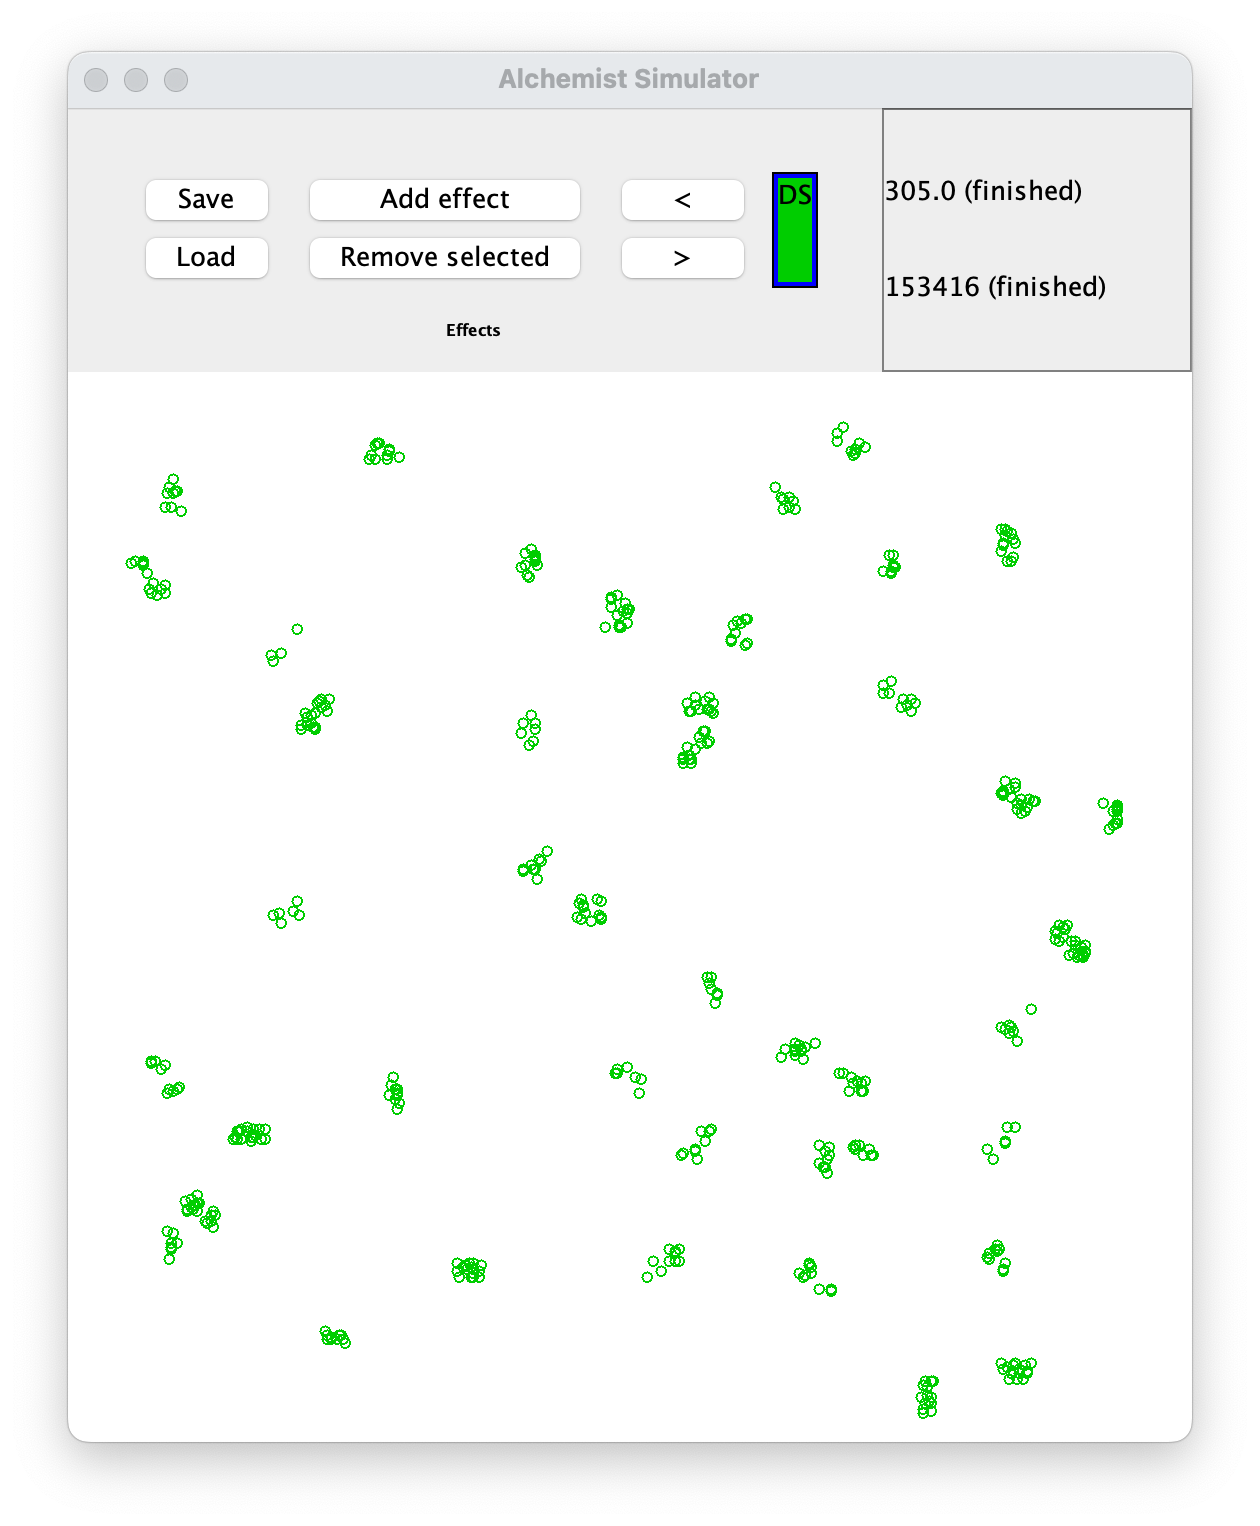
\includegraphics[width=0.32\textwidth]{figures/rectFine.png}}
    \caption{(a) Inizio (b) Dopo 100 secondi (c) Dopo 300 secondi}\label{fig:sim1}
\end{figure}
\begin{figure}[ht]
    \centering
    \subfigure[]{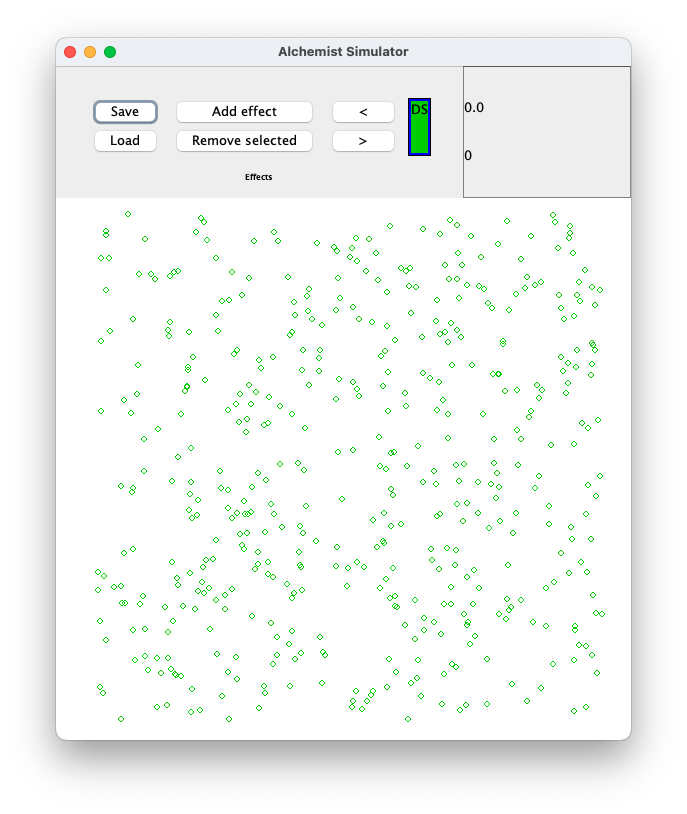
\includegraphics[width=0.32\textwidth]{figures/slow0.png}} 
    \subfigure[]{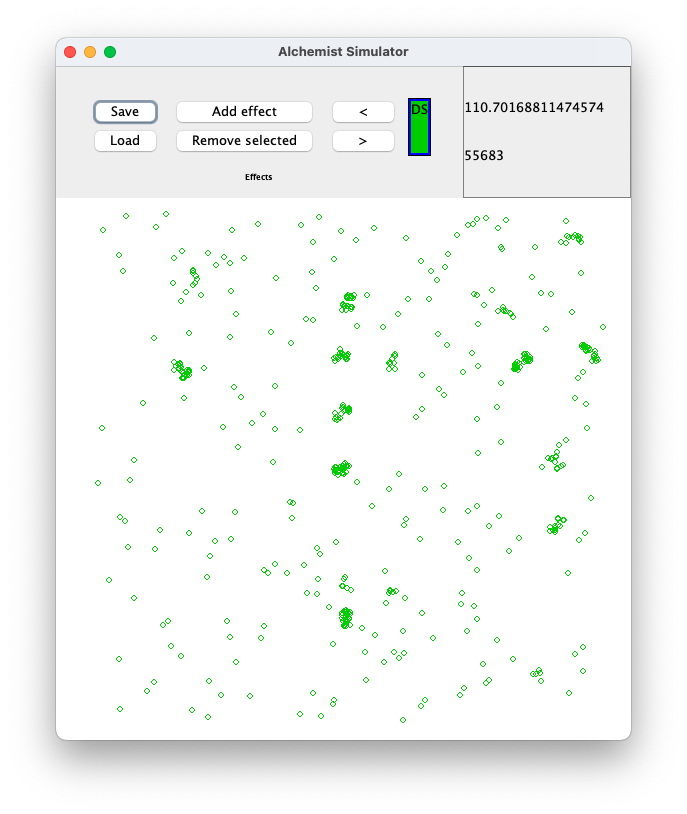
\includegraphics[width=0.32\textwidth]{figures/slow100.png}} 
    \subfigure[]{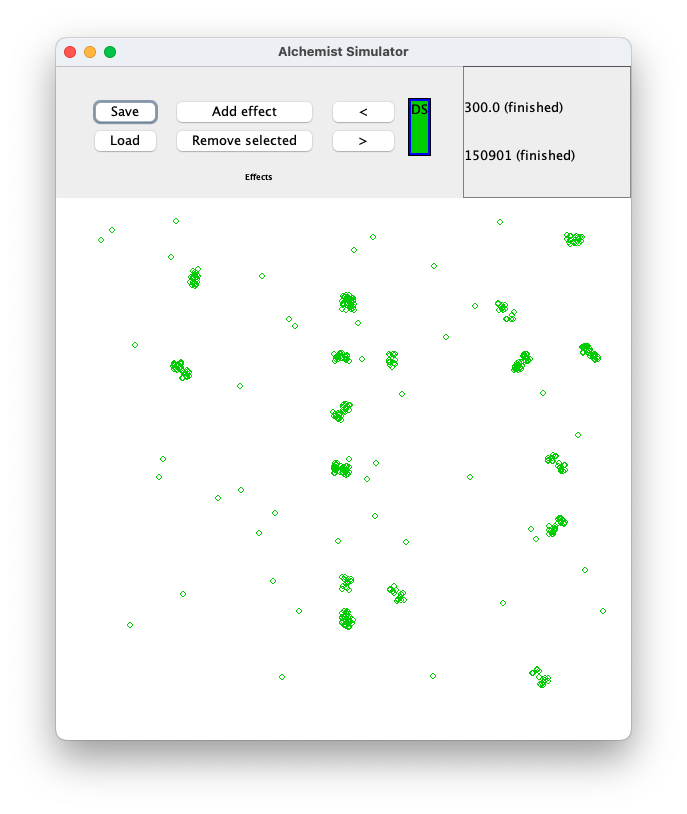
\includegraphics[width=0.32\textwidth]{figures/slowF.png}}
    \caption{(a) Inizio (b) Dopo 100 secondi (c) Dopo 300 secondi}\label{fig:sim2}
\end{figure}
\begin{figure}[ht]
    \centering
    \subfigure[]{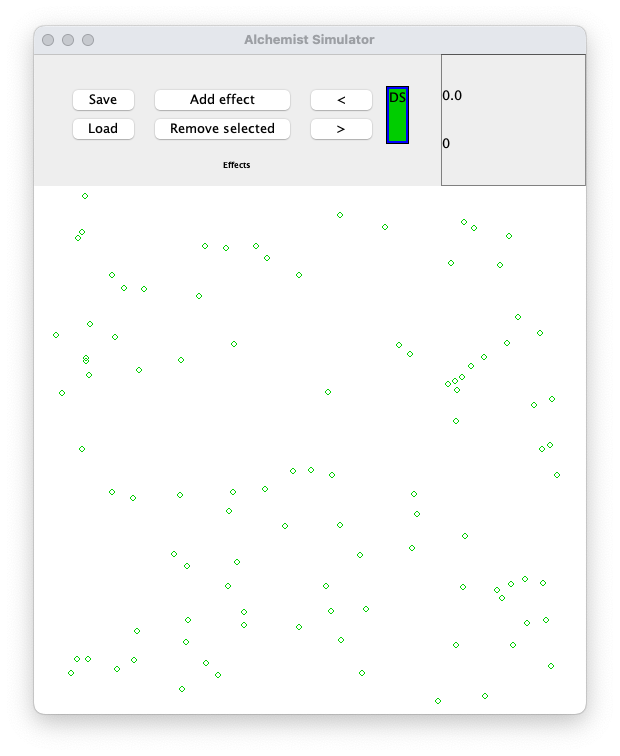
\includegraphics[width=0.32\textwidth]{figures/cento0.png}} 
    \subfigure[]{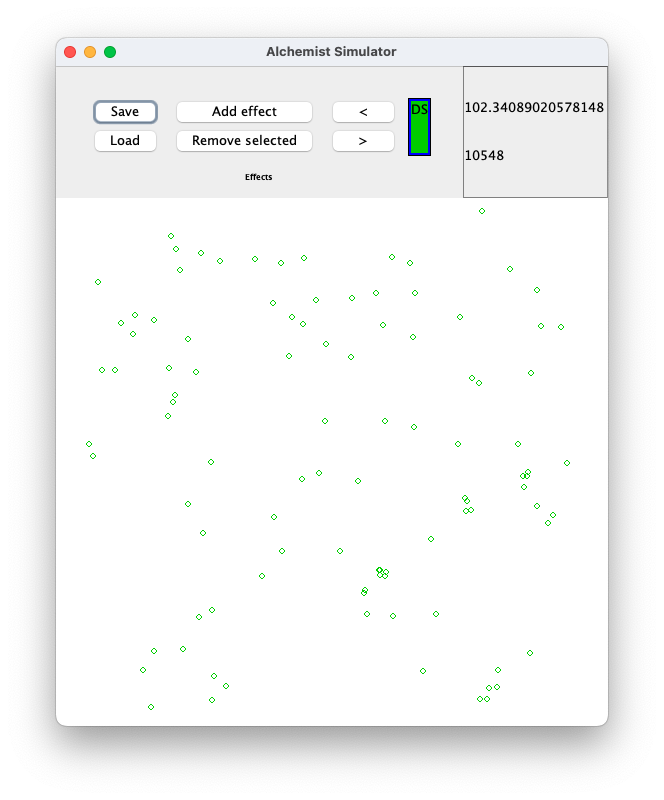
\includegraphics[width=0.32\textwidth]{figures/cento100.png}} 
    \subfigure[]{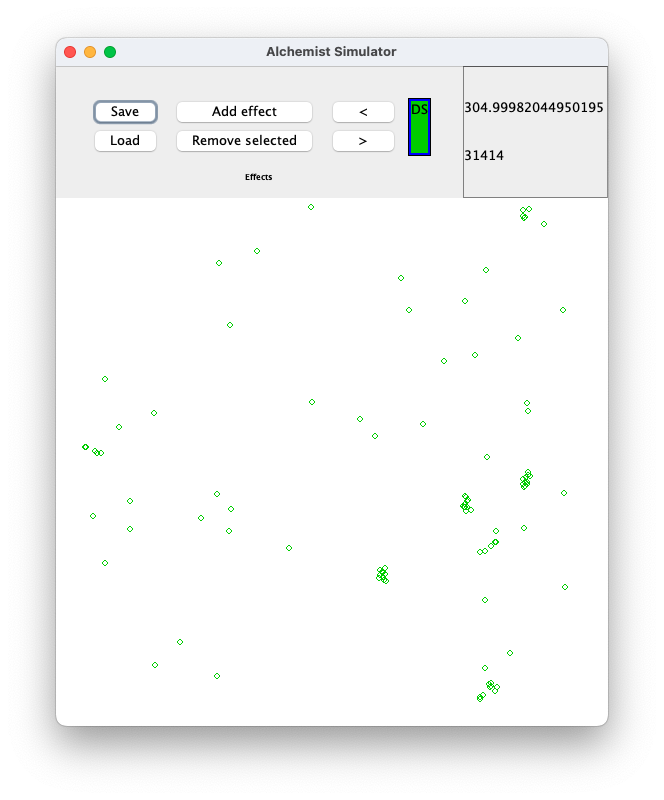
\includegraphics[width=0.32\textwidth]{figures/centoF.png}}
    \caption{(a) Inizio (b) Dopo 100 secondi (c) Dopo 300 secondi}\label{fig:sim3}
\end{figure}
\begin{figure}[ht]
    \centering
    \subfigure[]{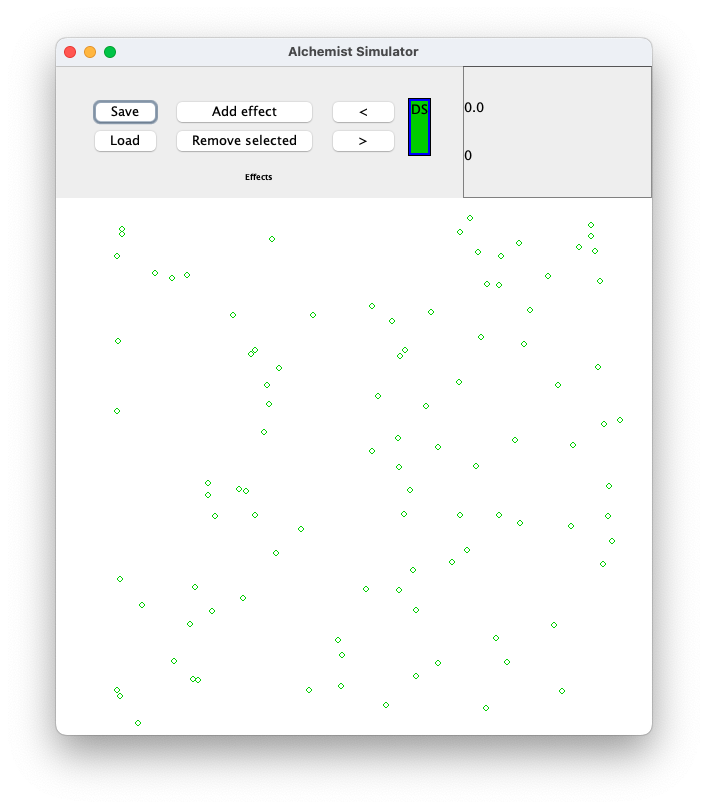
\includegraphics[width=0.32\textwidth]{figures/centoNo0.png}} 
    \subfigure[]{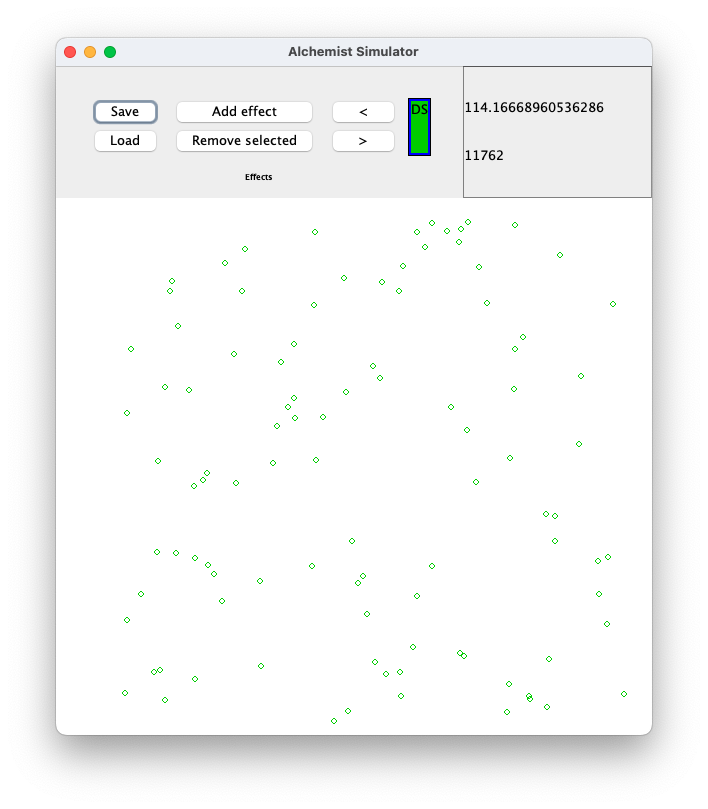
\includegraphics[width=0.32\textwidth]{figures/centoNo100.png}} 
    \subfigure[]{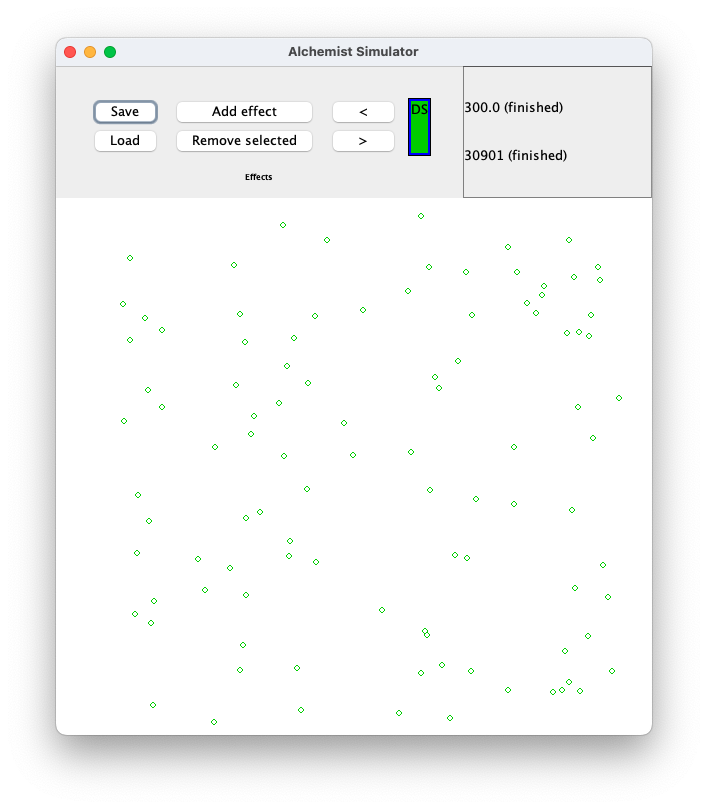
\includegraphics[width=0.32\textwidth]{figures/centoNoF.png}}
    \caption{(a) Inizio (b) Dopo 100 secondi (c) Dopo 300 secondi}\label{fig:sim4}
\end{figure}
\begin{figure}[ht]
    \centering
    \subfigure[]{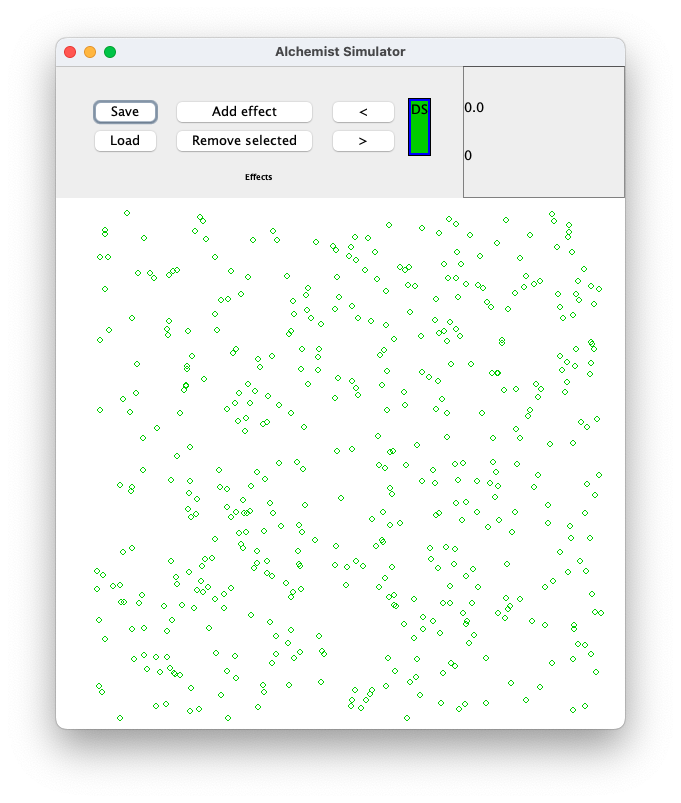
\includegraphics[width=0.32\textwidth]{figures/small0.png}} 
    \subfigure[]{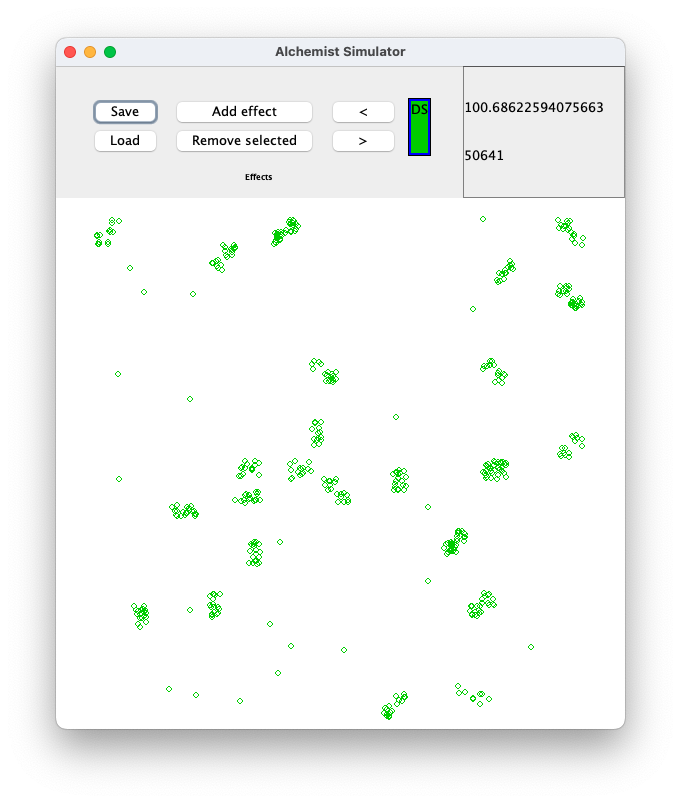
\includegraphics[width=0.32\textwidth]{figures/small100.png}} 
    \subfigure[]{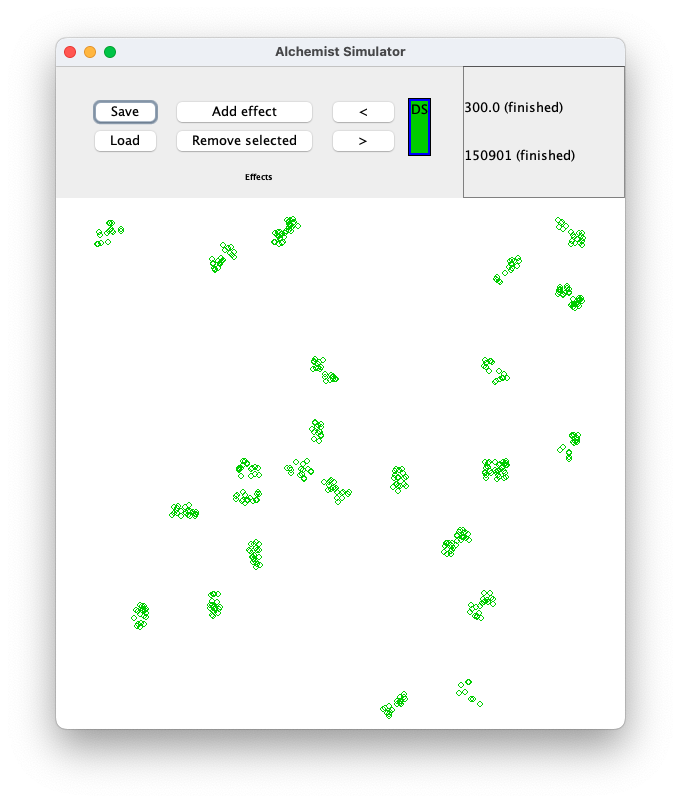
\includegraphics[width=0.32\textwidth]{figures/smallF.png}}
    \caption{(a) Inizio (b) Dopo 100 secondi (c) Dopo 300 secondi}\label{fig:sim5}
\end{figure}